\documentclass{article}

\usepackage[preprint]{neurips_2024}

\usepackage[utf8]{inputenc}
\usepackage[T1]{fontenc}
\usepackage{hyperref}
\usepackage{url}
\usepackage{booktabs}
\usepackage{amsfonts}
\usepackage{amsmath}
\usepackage{nicefrac}
\usepackage{microtype}
\usepackage{xcolor}
\usepackage{graphicx}

\title{Audio-Centric Visual Speech Reconstruction with Weak Text Conditioning}

\author{%
  DL-V2A Project Team \\
  \texttt{fm-avsr-cleanup} \\
}

\begin{document}
\maketitle

\begin{abstract}
This report summarizes the final audio generation method developed in the
FM-AVSR branch. The key finding is that high-quality visual speech audio
generation should not be treated as a strict
vision-to-text-to-audio cascade. In our final system, text is only a weak
semantic auxiliary condition; the main predictive path is from lip motion and
audio-derived latent conditions to continuous Mimi audio latents. This design
avoids making transcript accuracy the bottleneck. Replacing ground-truth text
with Auto-AVSR text changes full-validation latent correlation from 0.5818 to
0.5783, a drop of only 0.0035, while explicit timbre/audio prompt conditioning
and residual Mimi-latent reconstruction provide the major gains. The final
model uses Auto-AVSR visual features, SmolLM2 text hidden states, speaker
features, a 3.04-second Mimi audio prompt, and prompt-level timbre statistics
to reconstruct normalized Mimi latents. The strongest checkpoint reaches
0.58184180 mean correlation on the LRS3 validation split and supports raw-video
and silent-video inference with optional reference audio.
\end{abstract}

%======================================================================
\section{Goal and Main Claim}
%======================================================================

The project goal is to generate speech audio from talking-face video. The final
system is an offline research prototype: it predicts Mimi audio latents from
visual speech conditions and decodes them into waveform. It is not positioned as
a real-time product system or a full speaker-cloning model.

The central conclusion is architectural. A direct
\emph{vision $\rightarrow$ text $\rightarrow$ audio} pipeline is too dependent
on transcript quality and discards acoustic information that is visible in lip
dynamics but not represented by text. Our final route instead uses:
\begin{equation}
    \mathrm{lip/video} + \mathrm{weak\ text} + \mathrm{speaker/timbre}
    \longrightarrow \mathrm{Mimi\ audio\ latent}
    \longrightarrow \mathrm{waveform}.
\end{equation}
Text helps stabilize content, but it is not the main representation used to
generate audio. This explains why imperfect AVSR text can still produce
reasonable audio: the model is not forced to reconstruct speech from text
alone.

The final technical contributions are:
\begin{enumerate}
    \item \textbf{Audio-centric latent formulation.} We formulate visual speech
    generation as reconstruction of normalized continuous Mimi latents rather
    than as TTS from a transcript. This preserves acoustic information beyond
    text and gives a direct objective for waveform reconstruction.
    \item \textbf{Residual endpoint reconstruction architecture.} The final
    model abandons stochastic FM sampling for a deterministic endpoint predictor
    with a frozen base reconstructor and a learned residual correction.
    \item \textbf{Explicit timbre/audio prompt conditioning.} The first 38 Mimi
    frames, about 3.04 seconds, are used both as prompt tokens and as global
    mean/std timbre statistics. This provides speaker and recording-color cues
    that text cannot provide.
    \item \textbf{Weak text conditioning finding.} Ground-truth text and
    Auto-AVSR text give nearly identical latent correlation. This shows that, in
    this architecture, exact transcript accuracy is not the dominant bottleneck;
    the main load is carried by lip and audio-latent conditions.
    \item \textbf{Data processing as model evidence.} The final results depend
    on a consistent data representation: AVSR-compatible lip crops, Auto-AVSR
    visual latents/text, SmolLM2 hidden states, Mimi targets, speaker features,
    and prompt-derived timbre conditions.
\end{enumerate}

%======================================================================
\section{Data Processing and Data Use}
%======================================================================

Data construction is a core part of the method. Each clip is converted into a
matched set of visual, text, speaker, and audio-latent files. The model never
uses raw text alone as the generation target; all training and evaluation are
defined against Mimi continuous latents.

\subsection{Training and Validation Splits}

The final checkpoint is trained on the lip-AVSR processed pretrain split with
59,144 training clips and evaluated on a fixed 1,000-clip validation split:
\begin{itemize}
    \item train split:
    \path{configs/eval_splits/pretrain_lipavsr_train59144_seed44_plus_ready_remaining9144_excl_val1000_seed43.txt}
    \item validation split:
    \path{configs/eval_splits/pretrain_len80_260_lipavsr_val1000_seed43.txt}
\end{itemize}
Earlier 10k and 30k subsets were used to validate scale trends and ablations
before moving to the final 59k setting.

\subsection{Per-Clip Files}

\begin{table}[h]
\centering
\small
\begin{tabular}{@{}lll@{}}
\toprule
\textbf{File} & \textbf{Shape} & \textbf{Use in the model} \\
\midrule
\texttt{lip\_avsr.npy} & $(T_v,96,96)$ & AVSR-compatible grayscale mouth crop \\
\texttt{avsr\_enc\_lipavsr.npy} & $(T_v,768)$ & visual/lip condition \\
\texttt{avsr\_text\_lipavsr.txt} & text & Auto-AVSR transcript for raw inference \\
\texttt{smollm2\_h\_text\_json.npy} & $(L,960)$ & GT-text hidden states for in-domain eval \\
\texttt{smollm2\_h\_lipavsr.npy} & $(L,960)$ & AVSR-text hidden states for raw inference \\
\texttt{speaker\_emb.npy} & $(256)$ & face-based identity condition \\
\texttt{latent.npz} & $(T_a,512)$ & Mimi latent training target \\
\texttt{audio\_prompt.npy} & $(38,512)$ & Mimi prompt tokens, first 3.04 s \\
\texttt{timbre\_cond.npy} & $(1024)$ & prompt mean/std timbre condition \\
\bottomrule
\end{tabular}
\caption{Final per-clip representation. The model consumes conditions and
predicts the normalized Mimi latent target.}
\label{tab:data_files}
\end{table}

\subsection{Visual Processing}

The visual path must use the Auto-AVSR-compatible mouth crop
\texttt{lip\_avsr.npy}. The older RGB lip crop is not the final representation.
The correct crop is encoded by Auto-AVSR:
\begin{equation}
    e^{v}_{1:T_v} = \mathrm{AutoAVSR}_{\mathrm{enc}}(V_{\mathrm{lip}}),
    \qquad e^{v}_t \in \mathbb{R}^{768}.
\end{equation}
Auto-AVSR also produces a decoded text string. For external videos without
ground-truth text or timestamps, this decoded text becomes the text source.

This processing choice is important for generalization. On external raw videos,
switching from the old RGB lip path to the correct \texttt{lip\_avsr} path
improved latent correlation:
\begin{table}[h]
\centering
\small
\begin{tabular}{@{}lcc@{}}
\toprule
\textbf{Video} & \textbf{Old RGB lip path} & \textbf{Final lip-AVSR path} \\
\midrule
Trump & 0.30353260 & 0.38691377 \\
HRX   & 0.25592437 & 0.27240886 \\
\bottomrule
\end{tabular}
\caption{External-video checks showing why the final visual representation
matters. This is reported as data processing evidence, not as a standalone
contribution.}
\label{tab:external_visual}
\end{table}

\subsection{Audio Latent Target}

Mimi provides the continuous audio latent target. For each audio-latent frame
$z_t \in \mathbb{R}^{512}$, the training target is normalized per latent
dimension:
\begin{equation}
    y_t = \frac{z_t - \mu}{\sigma}.
\end{equation}
The model predicts $\hat{y}_{1:T}$, then denormalizes and decodes:
\begin{equation}
    \hat{z}_t = \hat{y}_t \sigma + \mu, \qquad
    \hat{x}_{\mathrm{wav}} = \mathrm{MimiDecoder}(\hat{z}_{1:T}).
\end{equation}
All reported MSE, MAE, and correlation metrics are computed in normalized Mimi
latent space, not waveform space.

\subsection{Text and Timbre Conditions}

Text is encoded by SmolLM2 into hidden states. For LRS3 validation with
ground-truth word timestamps, audio-latent frames are aligned to text positions
using word timestamps. For raw videos, timestamps are unavailable, so the hidden
states are uniformly resampled. This makes text usable even when it is not
perfectly recognized or perfectly aligned.

The timbre condition is derived from the first 38 normalized Mimi frames
$A \in \mathbb{R}^{38 \times 512}$:
\begin{equation}
    q = [\mathrm{mean}(A), \mathrm{std}(A)] \in \mathbb{R}^{1024}.
\end{equation}
The same $A$ is also provided as prompt tokens. Listening examples remove this
3.04-second prompt region when the prompt comes from the same clip, because the
first seconds are condition input rather than generated speech.

%======================================================================
\section{Architecture and Mathematical Formulation}
%======================================================================

\subsection{Condition Fusion}

Figure~\ref{fig:architecture} shows the final inference graph. The model
condition is:
\begin{equation}
    C = \{e^v_{1:T_v}, h_{1:L}, s, A, q\},
\end{equation}
where $e^v$ is the Auto-AVSR visual sequence, $h$ is the SmolLM2 text hidden
sequence, $s$ is the speaker embedding, $A$ is the audio prompt token sequence,
and $q$ is the prompt statistics timbre vector.

Auto-AVSR visual features are produced at about 25 Hz, while Mimi latents are
used at 12.5 Hz. The visual condition is aligned by taking every second visual
frame:
\begin{equation}
    v_t = e^v_{2t}.
\end{equation}

\begin{figure}[h]
    \centering
    
\includegraphics[width=\linewidth]{assets/system_architecture.png}
    \caption{Final audio-centric visual speech reconstruction architecture.
    Lip features, weak text hidden states, speaker identity, and audio-prompt
    timbre conditions are fused to predict normalized Mimi latents.}
    \label{fig:architecture}
\end{figure}

\subsection{Deterministic Residual Reconstruction}

The explored flow-matching route learned a vector field from noise to target.
It did not become competitive: sampling correlation stayed around 0.35, far
below the reconstruction route. The final model therefore fixes the inference
state to:
\begin{equation}
    \tilde{x}=0,\qquad \tau=1,
\end{equation}
and directly predicts the endpoint latent. There is no random noise input and
no iterative denoising loop.

The final checkpoint uses a frozen base reconstructor and a residual head:
\begin{equation}
    y_{\mathrm{base}} = f_{\mathrm{base}}(C), \qquad
    \Delta = f_{\mathrm{residual}}(C), \qquad
    \hat{y} = y_{\mathrm{base}} + \Delta.
\end{equation}
This residual design is the main architecture-level improvement because it
lets the final model refine a strong endpoint predictor instead of relearning
the whole mapping from scratch.

\begin{figure}[h]
    \centering
    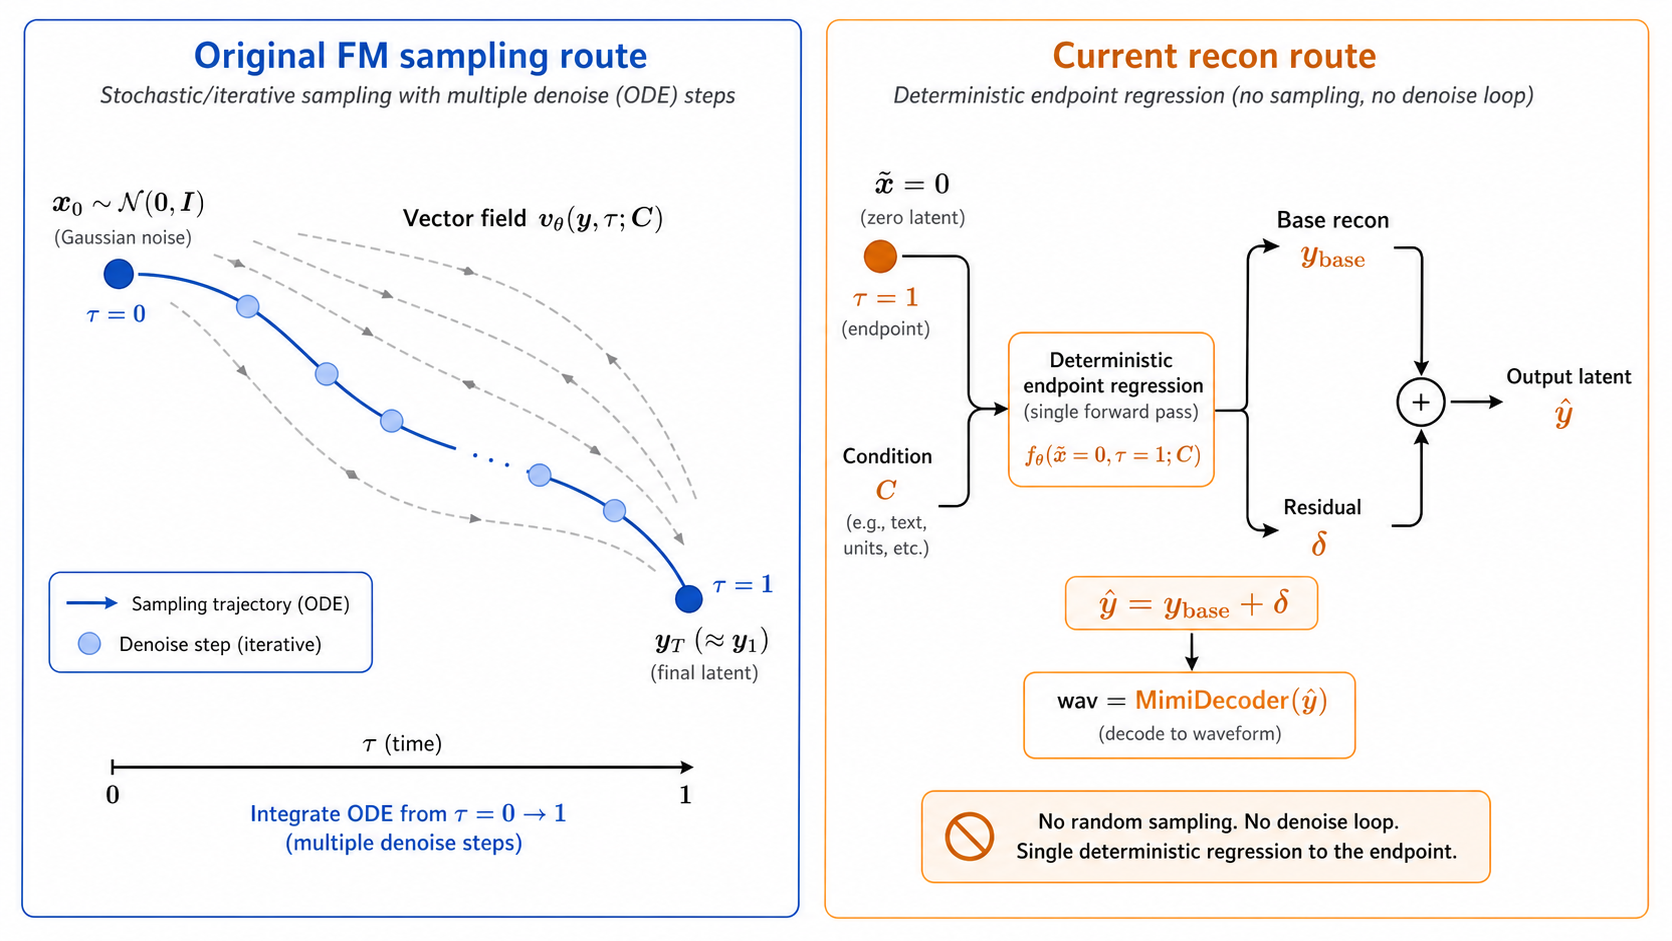
\includegraphics[width=\linewidth]{assets/recon_vs_sampling.png}
    \caption{The final route is deterministic endpoint reconstruction, not
    stochastic FM sampling. The model fixes $\tilde{x}=0$ and $\tau=1$, then
    predicts Mimi latents through a frozen base plus residual correction.}
    \label{fig:recon}
\end{figure}

\subsection{Training Objective}

The final loss combines reconstruction, sample-level correlation, and prompt
timbre statistics:
\begin{equation}
    \mathcal{L}
    = \mathcal{L}_{\mathrm{mse}}
    + 0.2\,\mathcal{L}_{\mathrm{corr}}
    + 0.05\,\mathcal{L}_{\mathrm{prompt\_stats}}.
\end{equation}
The correlation term is computed per clip after skipping the first 38 prompt
frames:
\begin{equation}
    \mathcal{L}_{\mathrm{corr}} =
    1 -
    \mathrm{corr}\left(
      \mathrm{vec}(\hat{y}_{39:T}),
      \mathrm{vec}(y_{39:T})
    \right).
\end{equation}
The prompt-statistics term encourages the generated segment to stay close to
the timbre statistics implied by the prompt.

%======================================================================
\section{Why Text Does Not Need to Be Exact}
%======================================================================

The final architecture treats text as an auxiliary semantic cue, not as the
central audio representation. This is a deliberate difference from a cascaded
vision-to-text-to-audio system.

In a cascade, recognition errors in the text stage directly become content
errors in the audio stage. In our model, lip motion and audio-latent prompt
conditions remain visible to the reconstructor. The text hidden state provides
coarse semantic guidance and helps stabilize alignment, but it does not have to
carry phonetics, speaker timbre, timing, and acoustic detail by itself.

The strongest evidence is the ground-truth text versus AVSR text evaluation:
\begin{table}[h]
\centering
\small
\begin{tabular}{@{}lrrr@{}}
\toprule
\textbf{Text condition} & \textbf{Corr} & \textbf{MSE} & \textbf{MAE} \\
\midrule
Ground-truth text + word timestamps
    & 0.58184180 & 0.66763106 & 0.60181897 \\
Auto-AVSR text
    & 0.57833471 & 0.67162028 & 0.60371083 \\
\bottomrule
\end{tabular}
\caption{Full LRS3 validation metrics on 1,000 clips. Replacing ground-truth
text with Auto-AVSR text drops correlation by only 0.00351.}
\label{tab:text_ablation}
\end{table}

This does not mean text is useless. It means transcript accuracy is not the
limiting factor in this architecture. Even when the text is imperfect, generated
audio can remain perceptually acceptable if the lip sequence and audio-latent
conditions are matched. Therefore, the project focus should remain on visual
speech representation, audio latent modeling, and timbre control rather than on
building a high-accuracy intermediate transcript.

The practical implication is important for system design. The text condition can
be noisy, and even substantial recognition errors should not be expected to
damage the audio in the same way they would damage a text-first cascade, because
the audio reconstructor still receives lip motion and audio-latent/timbre
conditions. We did not run a separate controlled word-error-rate sweep, so this
report does not claim a fixed WER threshold. The measured result is more
specific: replacing ground-truth text with the available Auto-AVSR text barely
changes the final latent metric.

%======================================================================
\section{Experimental Results}
%======================================================================

\subsection{Final Checkpoint}

\begin{itemize}
    \item \textbf{Config:}
    \path{configs/fm_avsr_lipavsr_59144_timbre3s_audioprompt38_pool_promptstats005_residual_samplecorr02_from1000_recon_textjson_wordts.yaml}
    \item \textbf{Checkpoint:}
    \path{runs/fm_avsr/lipavsr_59144_timbre3s_audioprompt38_pool_promptstats005_residual_samplecorr02_from1000_recon_textjson_wordts_v1/step_001500.pt}
    \item \textbf{Residual base:}
    \path{runs/fm_avsr/lipavsr_59144_timbre3s_audioprompt38_pool_from4000_recon_textjson_wordts_v1/step_005000.pt}
\end{itemize}

\subsection{Scale and Timbre Ablations}

\begin{table}[h]
\centering
\small
\begin{tabular}{@{}lrrr@{}}
\toprule
\textbf{Setup} & \textbf{Corr} & \textbf{MSE} & \textbf{MAE} \\
\midrule
10k visual-prior baseline & 0.50725122 & 0.77212131 & 0.65607136 \\
30k visual-prior baseline & 0.53081070 & 0.74379597 & 0.64330638 \\
30k no-timbre baseline & 0.53298334 & 0.72177195 & 0.63384026 \\
30k mean/std timbre & 0.56328889 & 0.68858632 & 0.61404544 \\
30k prompt tokens + pooled prompt + residual & 0.57255184 & 0.67793650 & 0.60844724 \\
Final 59k prompt-stats residual & 0.58184180 & 0.66763106 & 0.60181897 \\
\bottomrule
\end{tabular}
\caption{Main metric progression. Data scale improves the visual-prior model,
and timbre/audio prompt conditioning gives a larger gain than text-source
changes.}
\label{tab:main_progression}
\end{table}

The 10k to 30k scale-up improved matched validation correlation by about
0.0236. Timbre conditioning gave a larger change: the 30k no-timbre baseline
at 0.5330 moved to 0.5633 with mean/std timbre, and the prompt/residual route
reached 0.5726. The final 59k residual prompt-statistics checkpoint reached
0.5818.

The shifted-condition negative control for the 30k audio-prompt model dropped
to 0.00799 correlation, confirming that the model uses the matched conditions
rather than predicting an average latent.

\subsection{Raw and Silent Video Inference}

External raw-video inference uses Auto-AVSR text and uniform text alignment
because no ground-truth transcript or word timestamps exist. The final
raw-video path is therefore the same conceptual architecture as training, but
with the text source switched from \texttt{text\_json} to
\texttt{lipavsr}.

For silent video, the video supplies lip and face conditions while an optional
reference audio supplies $A$ and $q$. If no reference audio is provided, the
audio prompt and timbre vector are zero. The current demo export drops the
first 3.04 seconds because the model can copy reference-prompt audio into the
beginning of the generated waveform. This is a temporary export-time hack and
is listed as a model issue to fix.

\begin{figure}[h]
    \centering
    
\includegraphics[width=\linewidth]{assets/silent_ref_pipeline.png}
    \caption{Silent-video inference with optional reference audio. This is an
    application of the same audio-prompt/timbre conditioning mechanism used in
    training. Current listening exports skip the first 3.04 seconds to avoid
    reference-prompt leakage at the start.}
    \label{fig:silent_ref}
\end{figure}

%======================================================================
\section{Reproducibility Interfaces}
%======================================================================

The primary command-line entry point is:
\begin{verbatim}
python scripts/run_raw_video_avsr_recon_pipeline.py \
  --input data/trump.mov --exp trump_cleanup_verify --force
\end{verbatim}
For silent video with reference audio:
\begin{verbatim}
python scripts/run_raw_video_avsr_recon_pipeline.py \
  --input silent.mp4 --ref_audio ref.wav \
  --silent_input --exp demo --force
\end{verbatim}
The Gradio interface at \texttt{scripts/gradio\_avsr\_gui.py} exposes the same
backend with video upload, optional reference audio, and silent-input controls.

These interfaces are not counted as research contributions; they are included
so the result can be reproduced and demonstrated.

%======================================================================
\section{Limitations}
%======================================================================

\begin{itemize}
    \item The system is offline. Earlier timing showed that face alignment and
    lip cropping dominate runtime; the FM head and Mimi decoder are not the
    primary bottlenecks.
    \item The model is deterministic. It improves stability, but it can average
    speaker-specific acoustic detail, which explains some mixed-voice artifacts.
    \item Timbre control is based on prompt latents and prompt statistics. It is
    useful, but it is not equivalent to a high-fidelity speaker cloning model.
    \item The current silent-reference export skips the first 3.04 seconds
    because the model can copy prompt/reference audio at the beginning. A proper
    fix should prevent prompt leakage inside the model rather than relying on
    export-time cropping.
    \item External videos remain harder than LRS3 because of domain shift,
    crop quality, missing word timestamps, and imperfect Auto-AVSR text.
    \item Latent correlation is a useful paired-condition metric, but it is not
    a complete subjective audio-quality score.
\end{itemize}

%======================================================================
\section{Conclusion}
%======================================================================

The final FM-AVSR result is best understood as audio-centric visual speech
reconstruction. The model does not rely on a perfect intermediate transcript.
It uses lip evidence, weak text, speaker information, and audio-prompt timbre
conditions to reconstruct Mimi latents directly. The strongest empirical
evidence is that replacing ground-truth text with Auto-AVSR text only reduces
validation correlation by 0.0035, while timbre/audio-prompt conditioning and
residual endpoint reconstruction produce the major gains. This supports the
chosen architecture over a strict vision-to-text-to-audio cascade and identifies
future improvement targets: better lip/audio representations, stronger timbre
control, and higher-fidelity latent decoding.

\end{document}
